

\section{Introduction}


Recent Multimodal Large Language Models (MLLMs) have demonstrated strong performance on video understanding tasks, including action recognition \YSR{cite for each? we have several works, use those as well...}, temporal event localization, and video question answering. Existing action datasets have been highly effective in evaluating models across a wide range of everyday activities\cite{kinetics, ssv2, ucf101, hmdb51, activitynet}, sports actions \cite{multisports, finegym}, human-object interactions \cite{charades, actiongenome}, and complex temporal events \cite{momentsintime, multithumos}. While these tasks are important for general video understanding, reliable real-world systems must also recognize safety-critical behaviors, including physical altercations or threatening interactions. However, understanding aggression requires more than detecting that a violent or harmful action has occurred. In practical settings such as security, public safety monitoring, school safety, sports analysis, and online video moderation, it is often not enough to recognize what is happening; it is also necessary to understand how each person in the scene is involved. Without role-aware reasoning, a system may correctly classify a scene as aggressive while still producing an incorrect or harmful interpretation.

Prior work has studied aggressive actions through crime detection \cite{ucfcrimes, crxk}, violence detection \cite{xdviolence, cabad, moviesfight, violentflows, rwf, dvd, vid}, and incident understanding datasets \cite{iard, shanghaitech}. Some provide multiple aggressive action categories, while others formulate the task as binary classification, such as normal vs. anomalous or violent vs. non-violent. These resources have advanced the study of abnormal and dangerous events, but they typically evaluate only whether aggression is present. They often do not require reasoning about the individuals involved in the scene, including who initiates the action, or who is affected by it. In particular, existing evaluations rarely test whether an aggressive action can be bound to the correct actor, whether aggressors can be distinguished from victims and bystanders, or whether multi-person interactions can be resolved. This limitation can reward models that rely on contextual shortcuts, scene priors, or coarse motion cues, rather than learning the semantic relationships between people, actions, and roles. This necessitates a more fine-grained capability: \textbf{aggressive action and association}, where the goal is not only to recognize an aggressive behavior, but also to associate it with the correct participant roles.

To address this, we introduce A$^3$Bench, a benchmark for evaluating aggressive action and association in MLLMs. This contains 2,683 video clips and 15,004 video question-answer pairs designed to probe models beyond coarse aggression recognition. Instead of asking only whether a violent action occurs, our benchmark asks detailed questions about the type of aggressive action, and action-role relationships (aggressors, victims, bystanders). These questions require models to interpret the scene composition, distinguish the appearance between individuals, recognize and bind aggressive actions to the correct participants. By evaluating these fine-grained reasoning abilities, A$^3$Bench provides a focused testbed for assessing whether current MLLMs can reliably understand aggressive scenes at the level required for real-world deployment. Our experiments show that recent MLLMs struggle with this setting with most models achieving performance below 50\%. \RA{Talk about solution?}
\YSR{we should also add 1-2 interesting insights we have...}
\AB{Potential insights?:
(a) Aggressor bias: models systematically over-assign the aggressor role -- 37\% of true victims and 31\% of bystanders are mislabeled as aggressors, meaning a deployed system would routinely blame victims.
(b) Scale does not help: Qwen2.5-VL-72B (40.53\%) scores below several 8B models like Qwen3-VL-8B (46.96\%) and InternVL2.5-8B (45.77\%). A 10x parameter increase does not buy compositional aggression understanding.
(c) People without action: models identify the correct participant 30\% of the time while getting the action wrong, but the reverse (correct action, wrong person) is only 18\%. They find salient people but cannot determine what the aggression actually is.
(d) Reasoning is a dead end: thinking modes and CoT prompts average only 42.83\% overall, failing to outperform the best general-purpose model. Step-by-step reasoning does not fix the grounding deficit.
Recommendation: (a) + (b) together. aggressor bias is the most novel finding with real-world safety implications, and the scale result preempts the obvious ``just use a bigger model'' counterargument.}


Overall, our contributions are as follows:
\begin{itemize}
    
    \item We introduce A$^3$Bench, a benchmark of 2,683 video clips designed to evaluate fine-grained aggressive behavior understanding in MLLMs.
    
    \item We construct diverse question types of 15,004 video question-answer pairs for deep understanding by probing to role identification along with aggressive action understanding.
    
    \item We benchmark recent MLLMs revealing limitations in their ability to properly understand aggressive scenes.

    \item \RA{Solution?}
\end{itemize}

\begin{figure}[t!]
  \centering
    \centering
    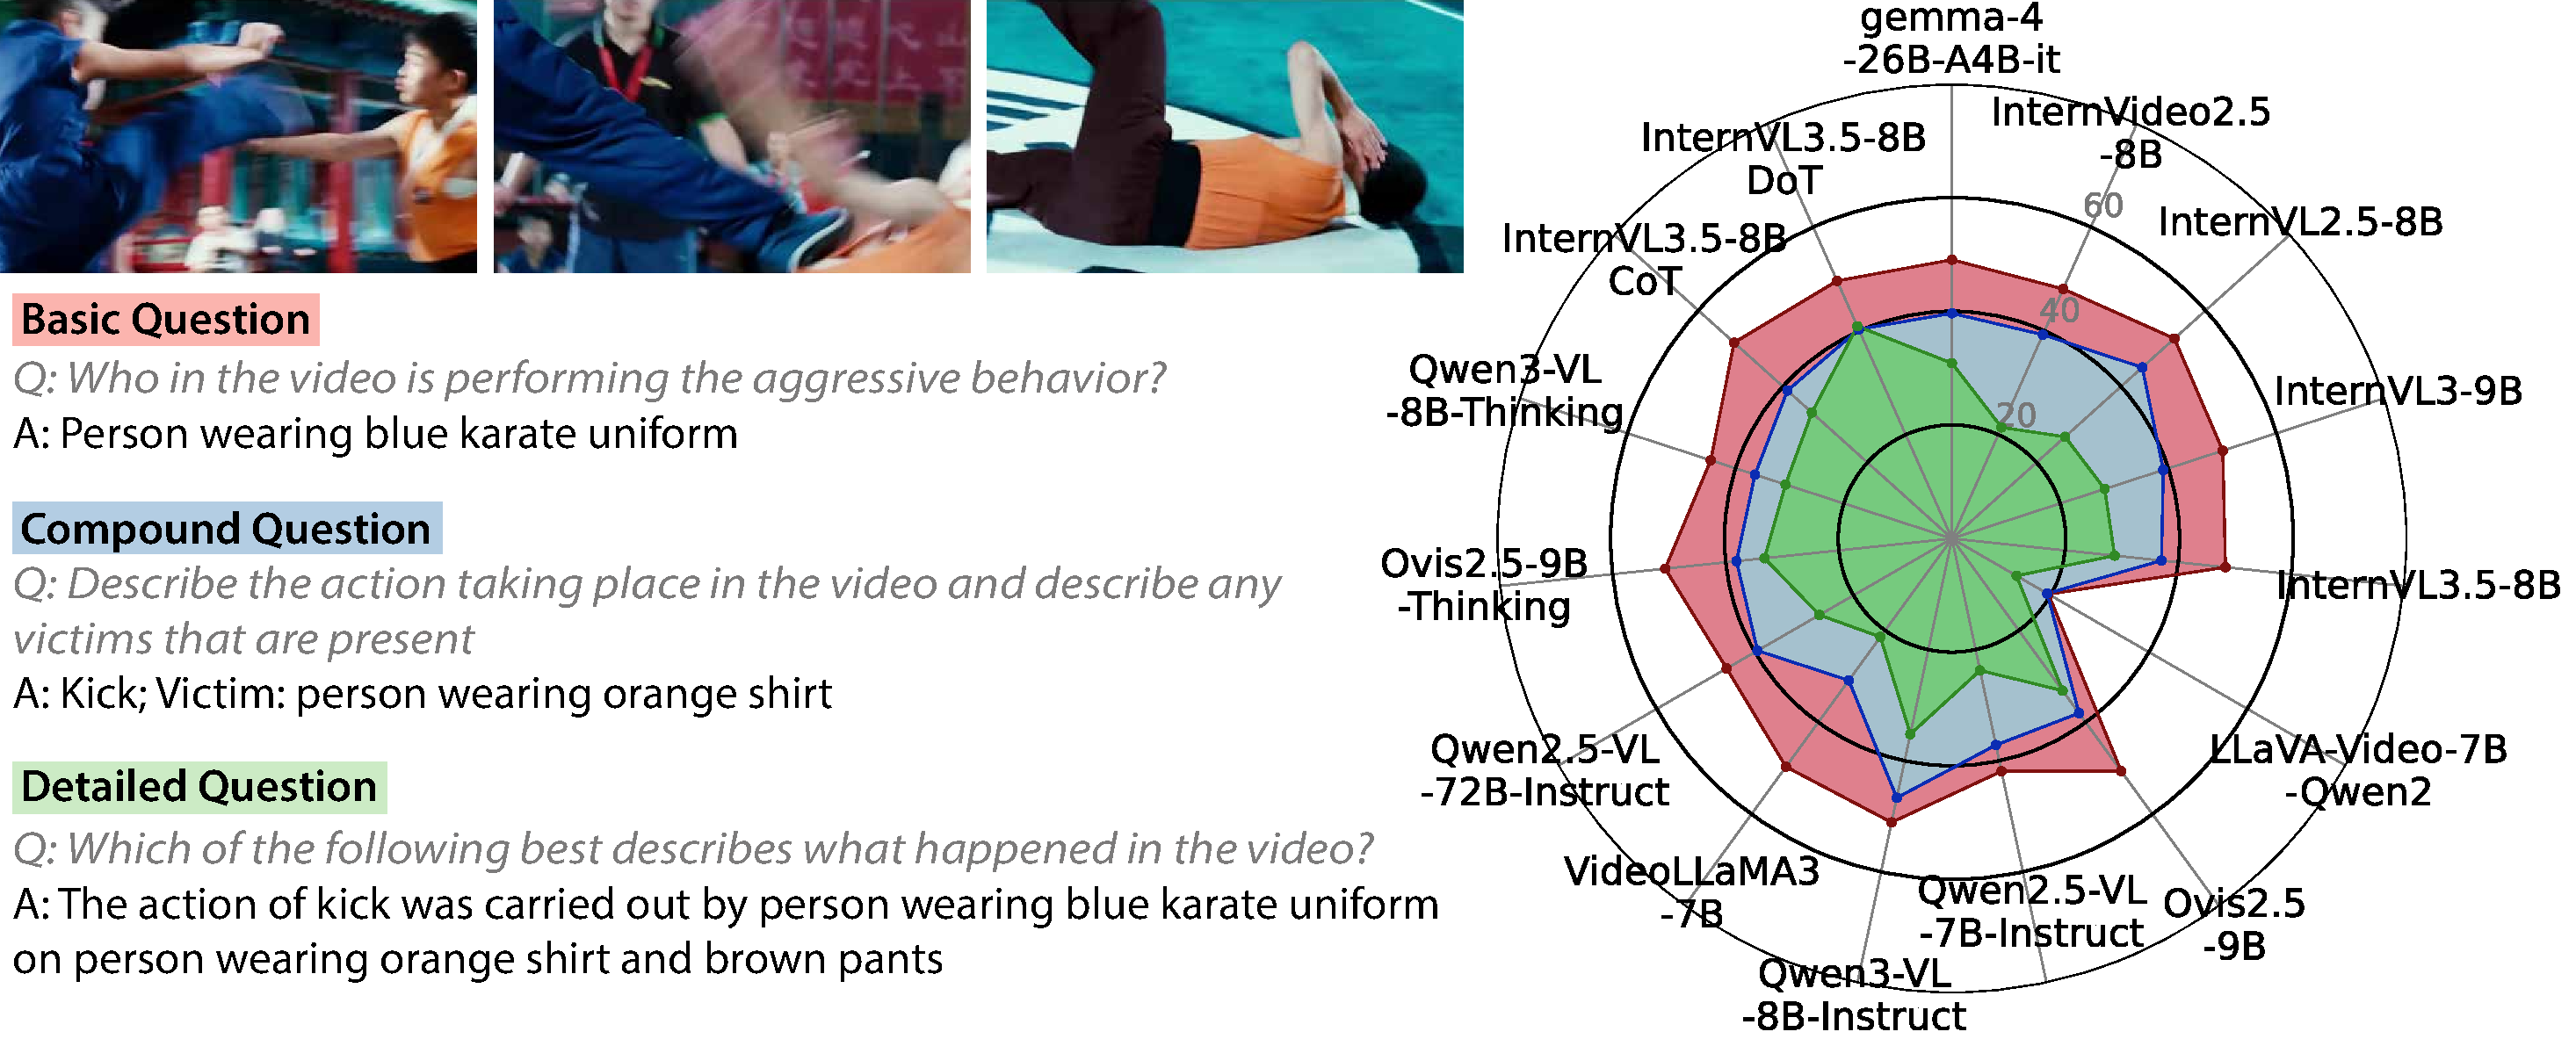
\includegraphics[width=\linewidth]{figures/teaser.pdf}
    
  \caption{\textbf{A$^3$Bench evaluates fine-grained aggressive action and association.}
\textit{Left:} Example question types. The benchmark progresses from basic questions that ask about a single attribute, to detailed questions that require understanding all aspects. \textit{Right:} Performance of evaluated MLLMs across the three question levels. Models perform poorly overall most scoring below 50\%, and accuracy decreases as the task becomes more difficult, with the lowest scores on detailed questions. This highlights the difficulty of moving from coarse aggression recognition to reliable actor-role and action binding.
\RA{reminder: need to update with GPT scores}
}

  \label{fig:teaser}
\end{figure}